\subsection{Morphology and Filtering}

After obtaining the foreground mask it's necessary to remove noise, consolidate certain 'blobs' and discard others. The GMM clusters pixels on their colour and how much it deviates from the accepted background model, thus darker pixels, in car windows in particular, can be classified as background pixels resulting into a series of disconnected components where only a single connected component should exist. In Figure \ref{fig:example_subtraction} a number of small foreground blobs often appear where a single vehicle exists in the corresponding original image, by applying morphology to the mask these blobs can be consolidated.

\subsubsection{Filtering}

Often salt and pepper noise can result from the subtraction process due to spurious lighting changes but by applying a median filter (\ref{subsection:median_filter}) it can be removed. Figure \ref{fig:foreground_mask_filtered} shows the effect of applying a median filter to remove noise from a foreground mask. It's important to remove this noise because firstly it's not a vehicle and secondly subsequent morphological operations may accentuate the noise and cause the system to generate incorrect output.


\subsubsection{Morphology}

Morphological operations are required to consolidate the foreground blobs that are disconnected when they should in fact be singular completely connected entities. This is important for the contouring process where an object is recognised by it's size and if a vehicle's foreground mask consists of a series of small disconnected blobs it will not be recognised. To consolidate these lonely blobs into a happy whole a morphological closing and dilation (\ref{section:morphology}) are performed the effect of which can be observed in Figure \ref{fig:foreground_mask_morphed}. The selection of structuring element shapes, size and number of iterations is dependent on the specific traffic scene presented and requires considerable calibration. 

\subsubsection{Calibration}

Generally, in at least one region of the foreground mask a superior formation of connected components straight out of the subtractor exists but there will always remain a number of disconnected components that require consolidation. By focusing on improving the consolidation of blobs in the aforementioned superior area this region can be exploited, furthermore, the counting and speed measuring operate only in a specific region where recognition and tracking is best. The reason that a single area must be selected and that object detection performance varies across an image is because of the camera's perspective of the traffic environment. If a camera is setup looking along the direction of movement of vehicles then their perceived size of said vehicles changes as they move closer and further from the camera. This affects numerous factors in the detection process but in the case of morphology it means that the features of vehicles that cause them to result in a fractured foreground mask, notably their windows and wheels which look similar to road from the perspective of the background subtractor, have variable size depending on the vehicle's distance from the node. Hence, the structuring element used for augmenting the foreground mask should match the scale of the disconnection in entities which is determined by the region of interest specified by the natural performance of the background subtractor. 

To find the optimal morphological structuring element shape, size and number of iterations requires greater testing than selecting a median filter. These operations can become computationally expensive depending on the size of the structuring element and number of iterations so minimising these factors is important. The OpenCV function, \emph{exmorphology} provides three shapes of structuring element, ellipse, cross and rectangle and Figure \ref{fig:morph_testing} shows the comparative performance of these shapes on the same foreground mask for a 7x7 element size and varying iterations. Visual analysis of foreground entities consolidation reveals that the rectangular element for 3 iterations performs the best in the area of the mask where the best connection and separation of vehicle masks is already occurring. Figure \ref{fig:compare_closure} highlights one example of connecting blobs where other methods failed, in this case the blobs in the bounding boxes are closed successfully by the rectangular structuring element but not by the ellipse.

\begin{figure}[H]
    \centering
    \begin{subfigure}[b]{0.45\textwidth}
        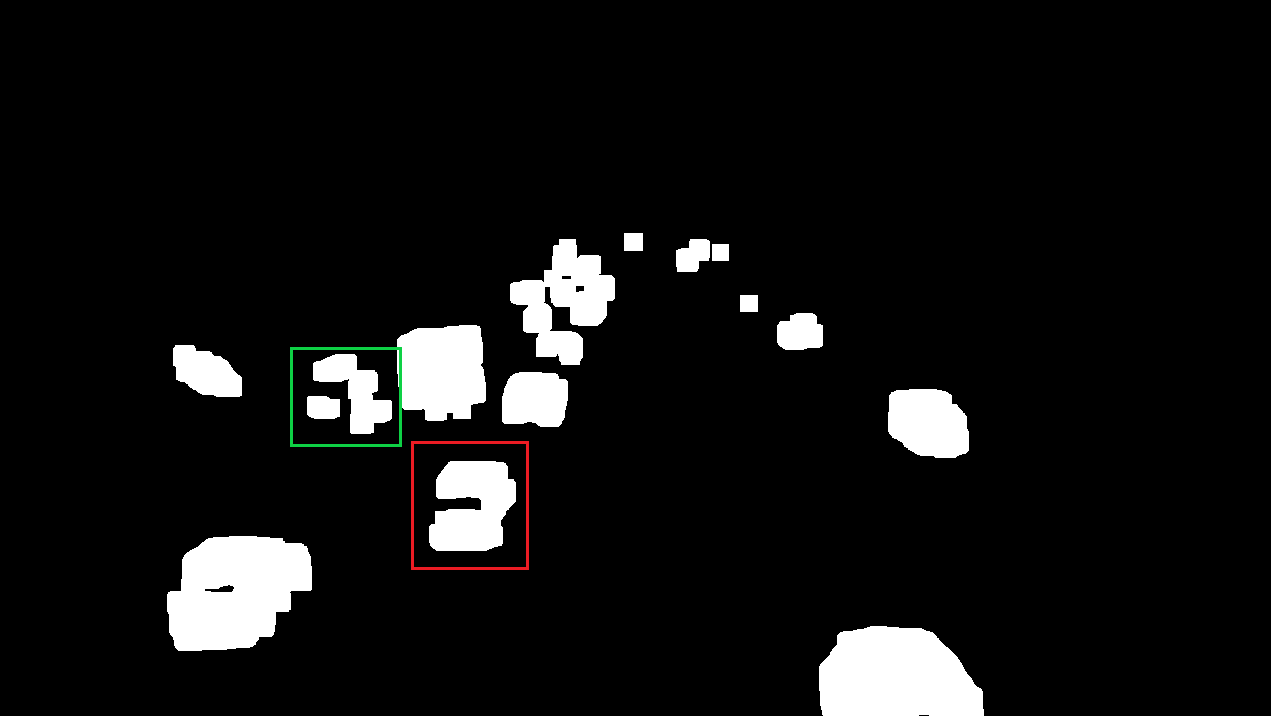
\includegraphics[width=\textwidth]{design/detection/calibration/rect_3_edit}
        \caption{Closure with rectangle.}
    \end{subfigure}
    \begin{subfigure}[b]{0.45\textwidth}
        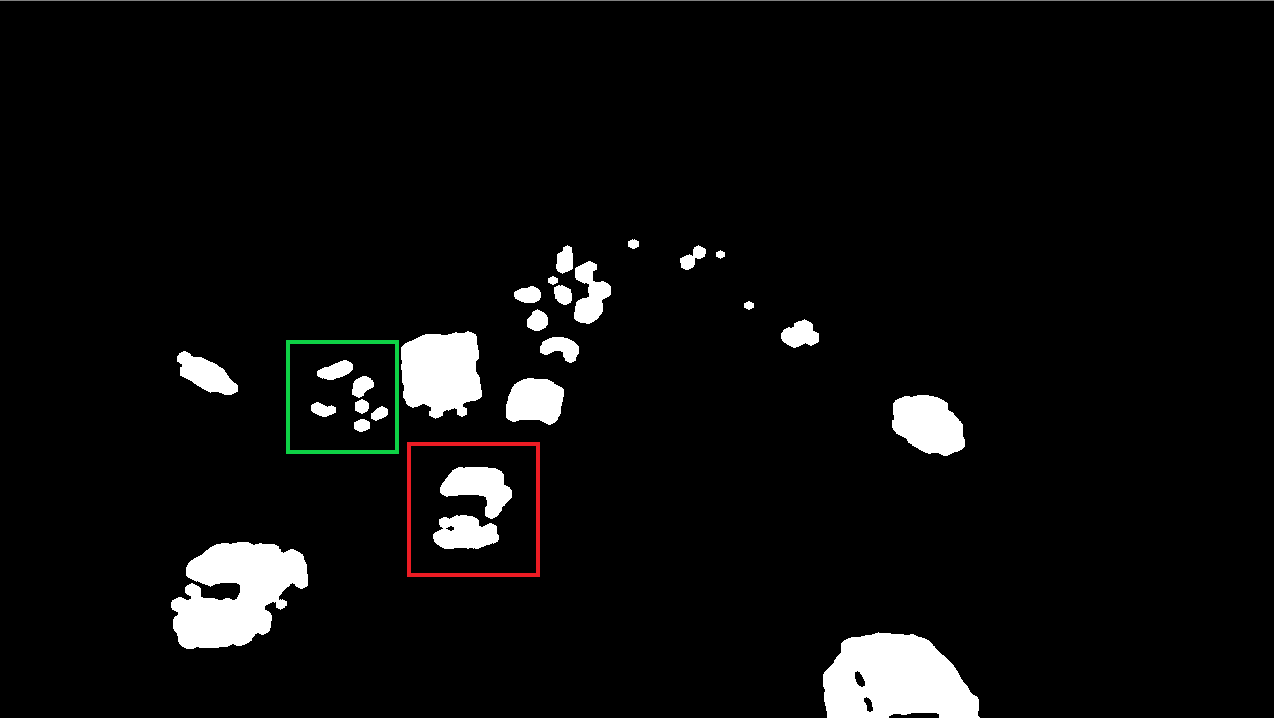
\includegraphics[width=\textwidth]{design/detection/calibration/ellipse_3_edit}
        \caption{Closure with ellipse.}
    \end{subfigure}
    \captionsetup{format = hang}
    \caption{Comparison of morphological closure using a 7x7 rectangular and elliptical structuring element for 3 iterations.}
    \label{fig:compare_closure}
\end{figure}


\begin{figure}[H]
    \begin{tabular}{
        >{\centering\arraybackslash}m{0.4cm}
        >{\centering\arraybackslash}m{4.5cm}
        >{\centering\arraybackslash}m{4.5cm}
        >{\centering\arraybackslash}m{4.5cm}}
          & Ellipse & Cross & Rectangle \\
        1 
        &
        \begin{subfigure}[b]{0.3\textwidth}
            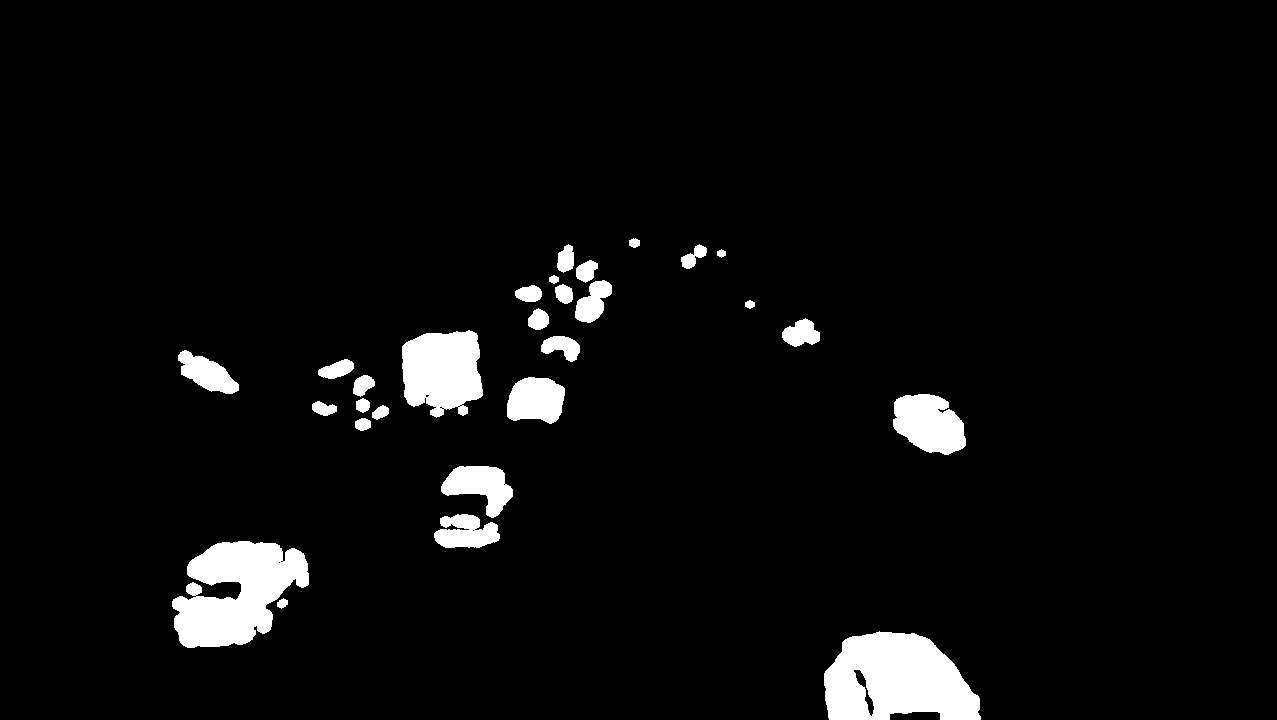
\includegraphics[width=\textwidth]{design/detection/morphology/ellipse_1}
            % \captionsetup{format = hang}
        \end{subfigure} &
        \begin{subfigure}[b]{0.3\textwidth}
            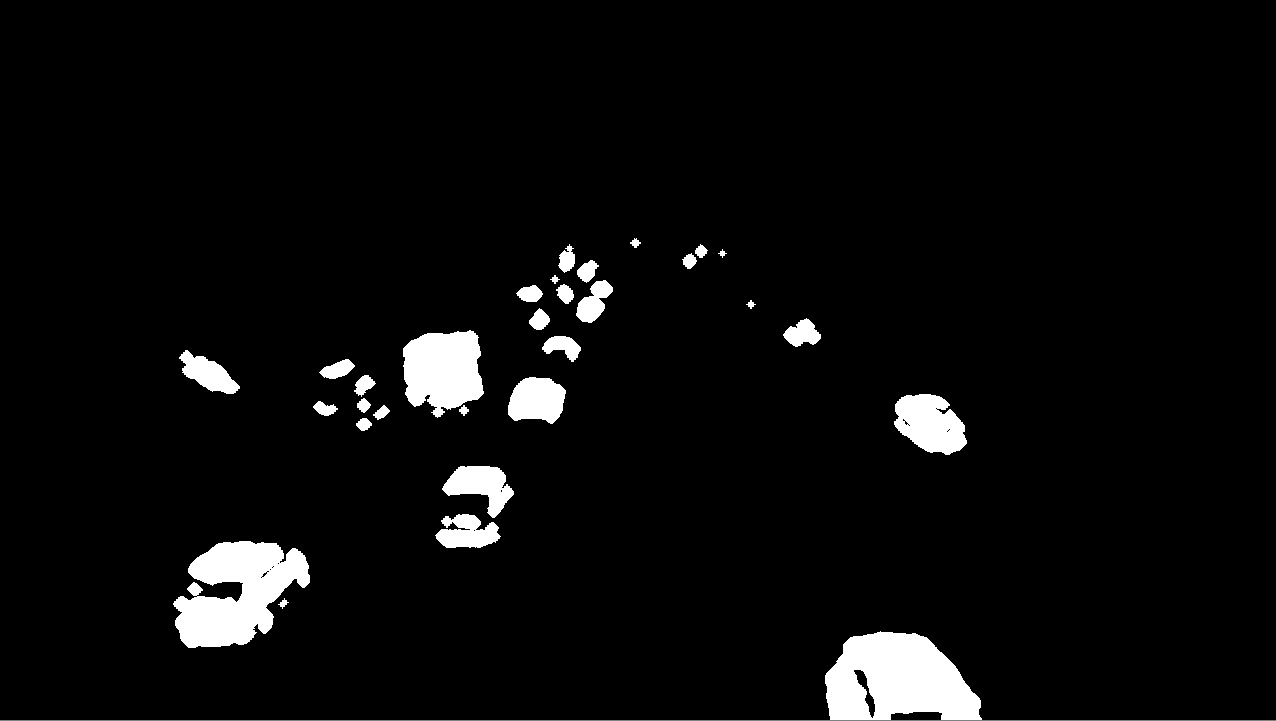
\includegraphics[width=\textwidth]{design/detection/morphology/cross_1}
            % \captionsetup{format = hang}
        \end{subfigure} &
        \begin{subfigure}[b]{0.3\textwidth}
            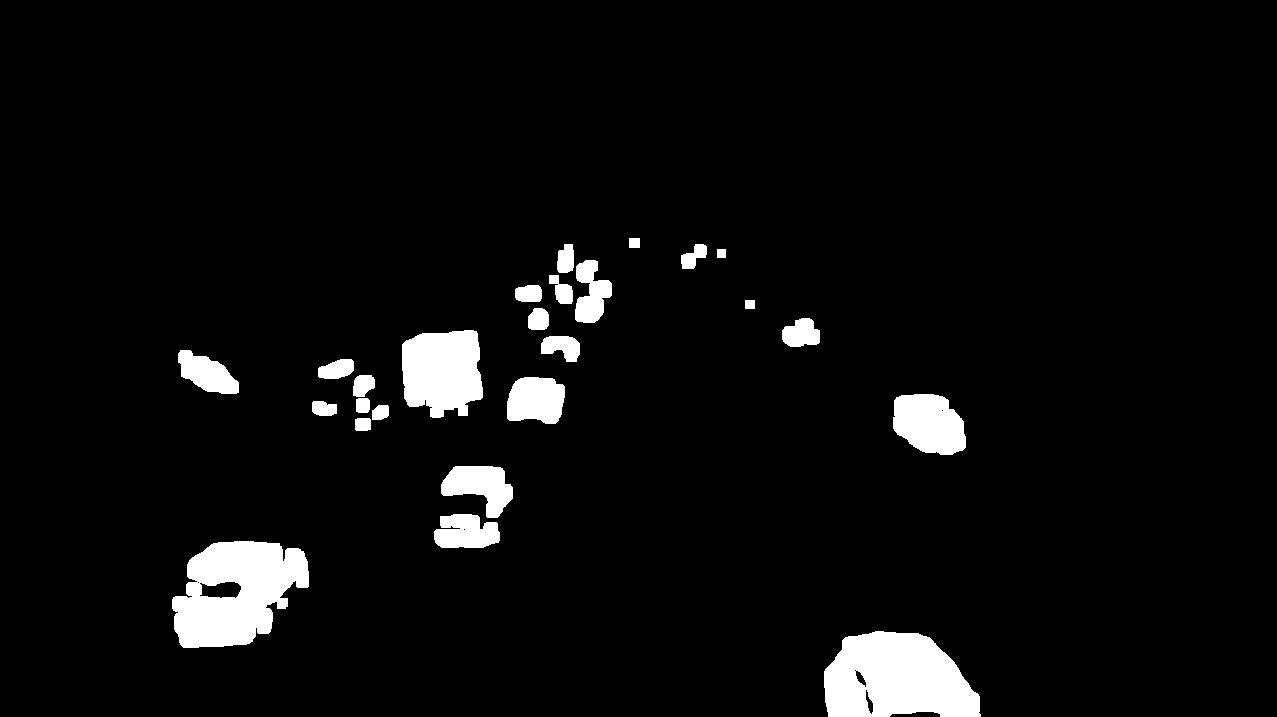
\includegraphics[width=\textwidth]{design/detection/morphology/rect_1}
            % \captionsetup{format = hang}
        \end{subfigure} \\
        3 &
        \begin{subfigure}[b]{0.3\textwidth}
            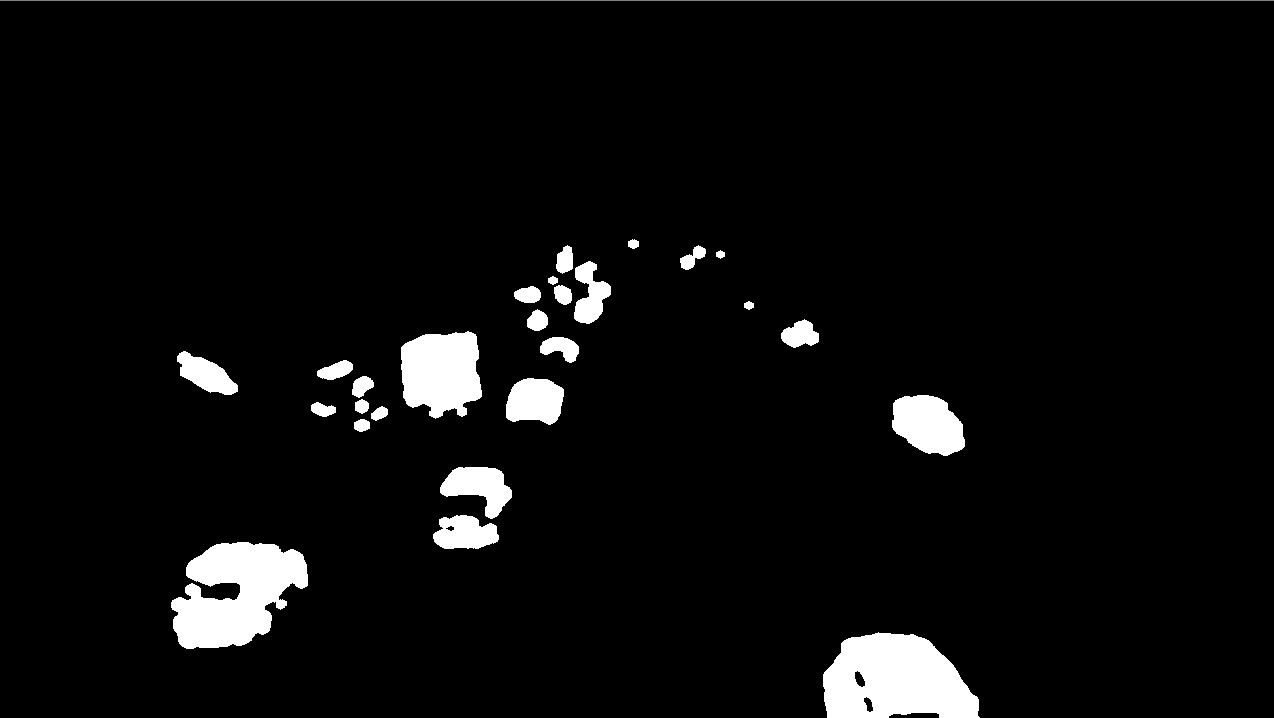
\includegraphics[width=\textwidth]{design/detection/morphology/ellipse_3}
            % \captionsetup{format = hang}
        \end{subfigure} &
        \begin{subfigure}[b]{0.3\textwidth}
            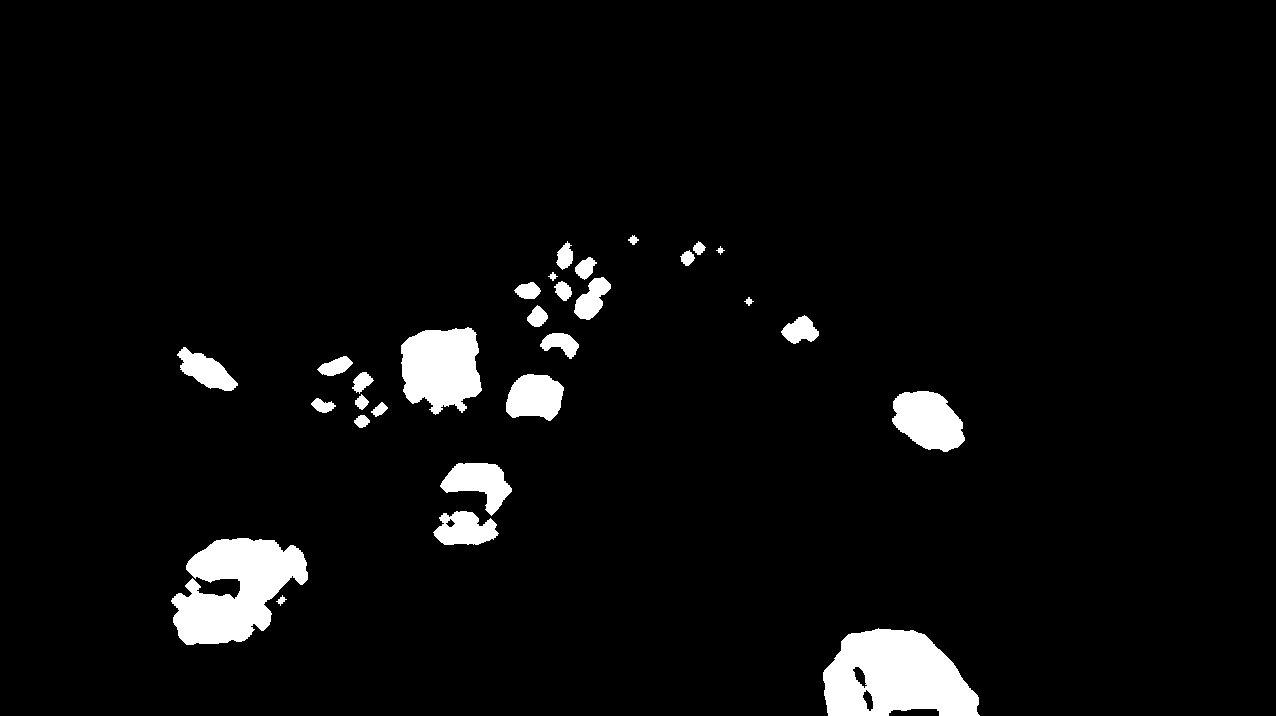
\includegraphics[width=\textwidth]{design/detection/morphology/cross_3}
            % \captionsetup{format = hang}
        \end{subfigure} &
        \begin{subfigure}[b]{0.3\textwidth}
            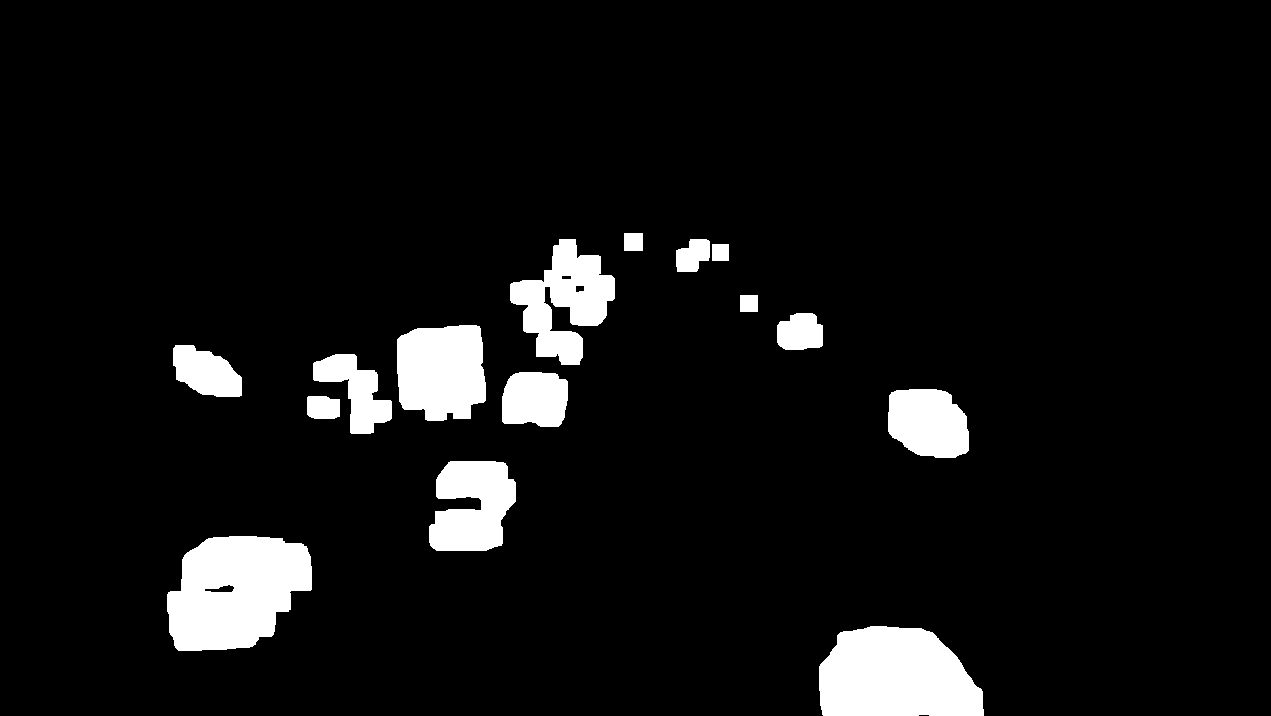
\includegraphics[width=\textwidth]{design/detection/morphology/rect_3}
            % \captionsetup{format = hang}
        \end{subfigure} \\
        5 &
        \begin{subfigure}[b]{0.3\textwidth}
            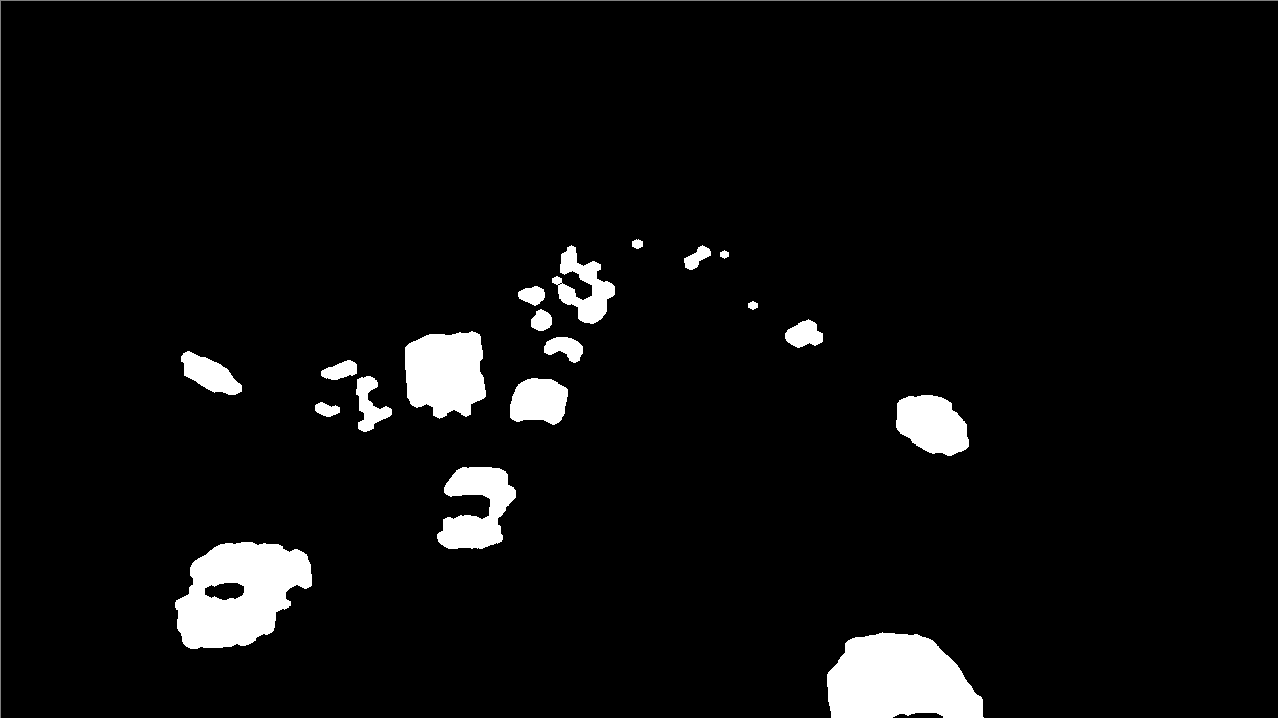
\includegraphics[width=\textwidth]{design/detection/morphology/ellipse_5}
            % \captionsetup{format = hang}
        \end{subfigure} &
        \begin{subfigure}[b]{0.3\textwidth}
            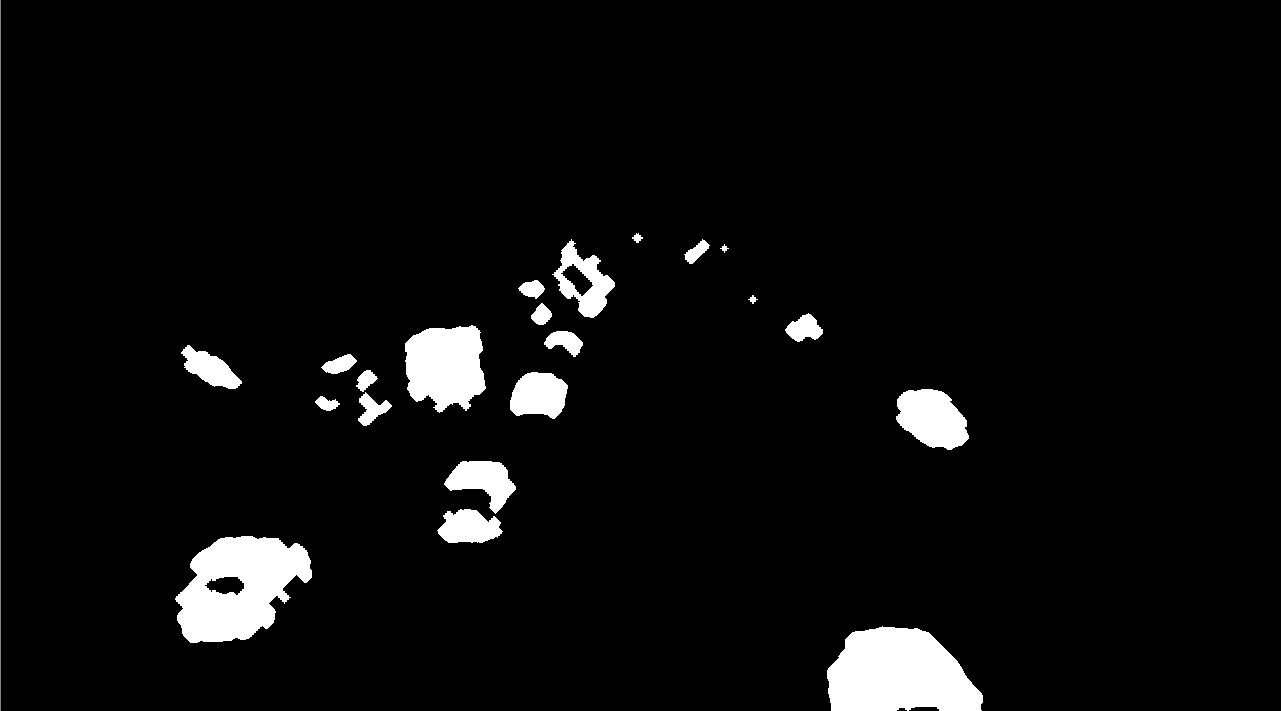
\includegraphics[width=\textwidth]{design/detection/morphology/cross_5}
            % \captionsetup{format = hang}
        \end{subfigure} &
        \begin{subfigure}[b]{0.3\textwidth}
            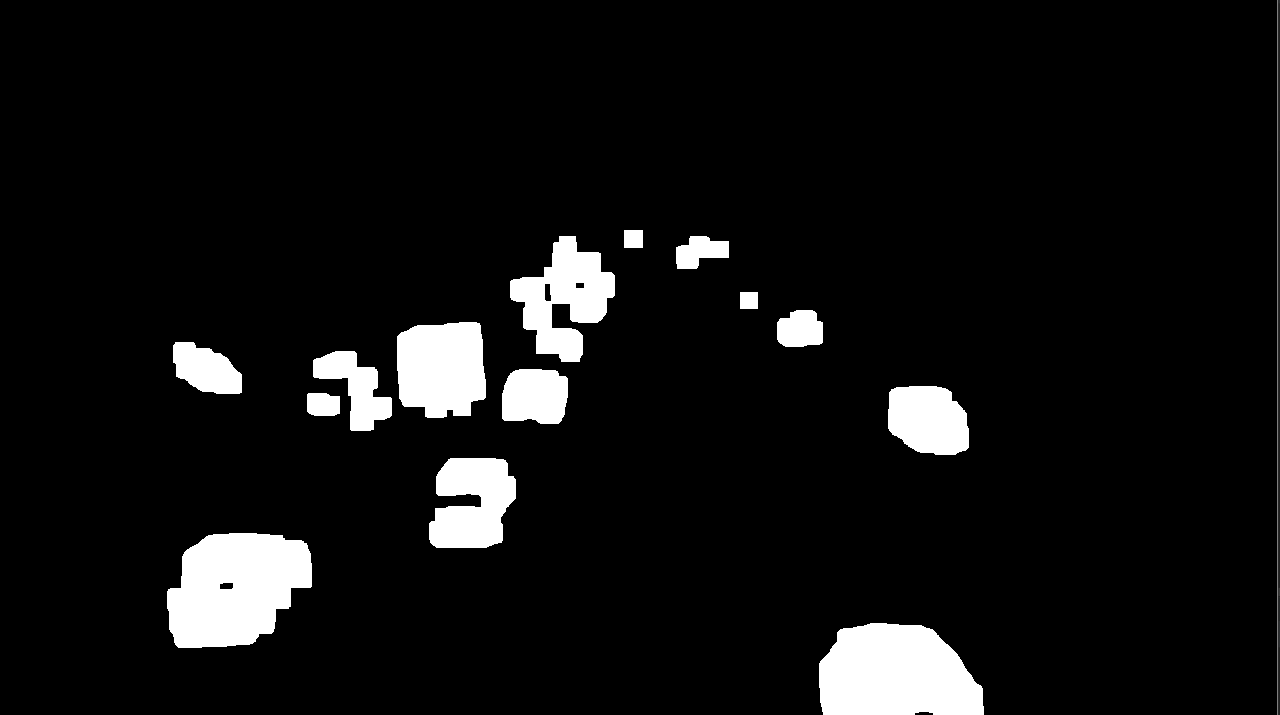
\includegraphics[width=\textwidth]{design/detection/morphology/rect_5}
            % \captionsetup{format = hang}
        \end{subfigure} \\
    \end{tabular}
    \captionsetup{format = hang}
    \caption{Morphological closing using different 7x7 structuring elements and iterations.}
    \label{fig:morph_testing}
\end{figure}
